\section{Introduction}


\subsubsection*{Problem Statement}

%What: The need of edge computing to enable low latency and mobile computation offloading
With the advent of Internet of Things, the evolution of mobile computing, and the emergence of real-time applications, the processing of an exponentially increasing volume of data must be performed in a timely fashion, i.e., with minimum latency. Despite the elasticity and vast computing power of existing cloud platforms, the access to these resources involves multiple hops of network communication, adding prohibitive latency to requests' processing. Such limitation has the following implications: 1) cloud services may fail to satisfy the requirements of real-time/low-latency applications; and 2) offloading of delay-sensitive computation from devices with constrained resources to cloud servers is unlikely to work due to network-latency.

%What: The challenges in realizing edge computing
To reduce network latency, data processing must be performed closer to where it is produced and consumed. In accordance with this principle, the emerging paradigm of edge computing~\cite{Shi:2016} states that computing power should be pushed from centralized datacenters to the edge of the network. 
%What: The challenges in the realization of edge computing
The materialization of this paradigm, however, still poses many challenges:

%What: Resouce limitations of edge computing and the need for a more efficient provisioning
%What: Aways availability vs opportunistic service setup
--- First, a finely distributed edge infrastructure~\cite{Dehos14millimeter5g} is not expected to exhibit virtually unlimited resources as cloud datacenters. This limitation imposes a more efficient allocation of edge resources. Current models based on virtualization and containerization, although successfully adopted by cloud providers, may not be feasible in the context of edge computing, as they require a minimum pre-allocation of resources. Therefore, a different execution model is needed to deem edge computing scalable~\cite{GarrigaMendonca2017}. Also, while cloud services cover very large areas in which requests from clients are always expected, the fine-grained coverage of edge computing implies that services would remain idle whenever clients are absent, while other services may lack sufficient resources. Therefore, to optimize the usage of edge resources, services should be opportunistically made available.

%What: The need for taking alternative edge domains into account
--- Second, different sorts of edge computing infrastructures may exist~\cite{1,2,Tarneberg2017}, including servers located at cellular base stations, temporarily placed nearby public events, and inside buildings and houses to provide support for smart space applications. Edge servers that are integrated to local network infrastructures would require the discovery of edge services on-the-fly when inside their coverage area.

%What: The continuum
--- Finally, considering that edge-based services may not always be available and taking into account the high availability of cloud-based services, the former should complement rather than replace the later. This vision also extends to computation that may opportunistically be offloaded from resource-constrained devices to nearby edge servers in order to augment their capabilities. In this sense, cloud, edge, and mobile computing should be seen as parts of a \textit{computational continuum} serving different sorts of applications. Its realization requires not only the materialization of edge computing,
%, whose particular characteristics require an \textit{efficient} management and provisioning of its resources, 
but also the mechanisms to allow computation to be seamlessly placed onto the heterogeneous parts composing the continuum according to dynamic contexts of clients and servers. % including both the context of clients and service providers.




%Also, the eventual co-existence of alternative service providers would require the client-side participation on the placement of computation along the continuum~\cite{Soyata:2012,Tarneberg2017}, which requires the awareness of alternative services by clients.

Fig.~\ref{fig:continuum-overral} describes the different parts composing the cloud-edge-mobile continuum. Cloud computing features virtually unlimited computational resources and shall remain as the source of services with higher availability. Edge computing, in turn, features low network latency and shall provide services for real-time and delay-sensitive applications. Finally, despite the improvements in the capabilities of mobile devices, the later still suffer from battery drain and other platform/hardware limitations which motivates computation offloading. In addition to the commonly employed mobile-cloud inter-operation, mobile devices can integrate the continuum as both clients of computation that may opportunistically be offloaded to edge servers and providers of their own local services to cope with the situations in which edge is not available. 

\begin{figure}[tbp]
	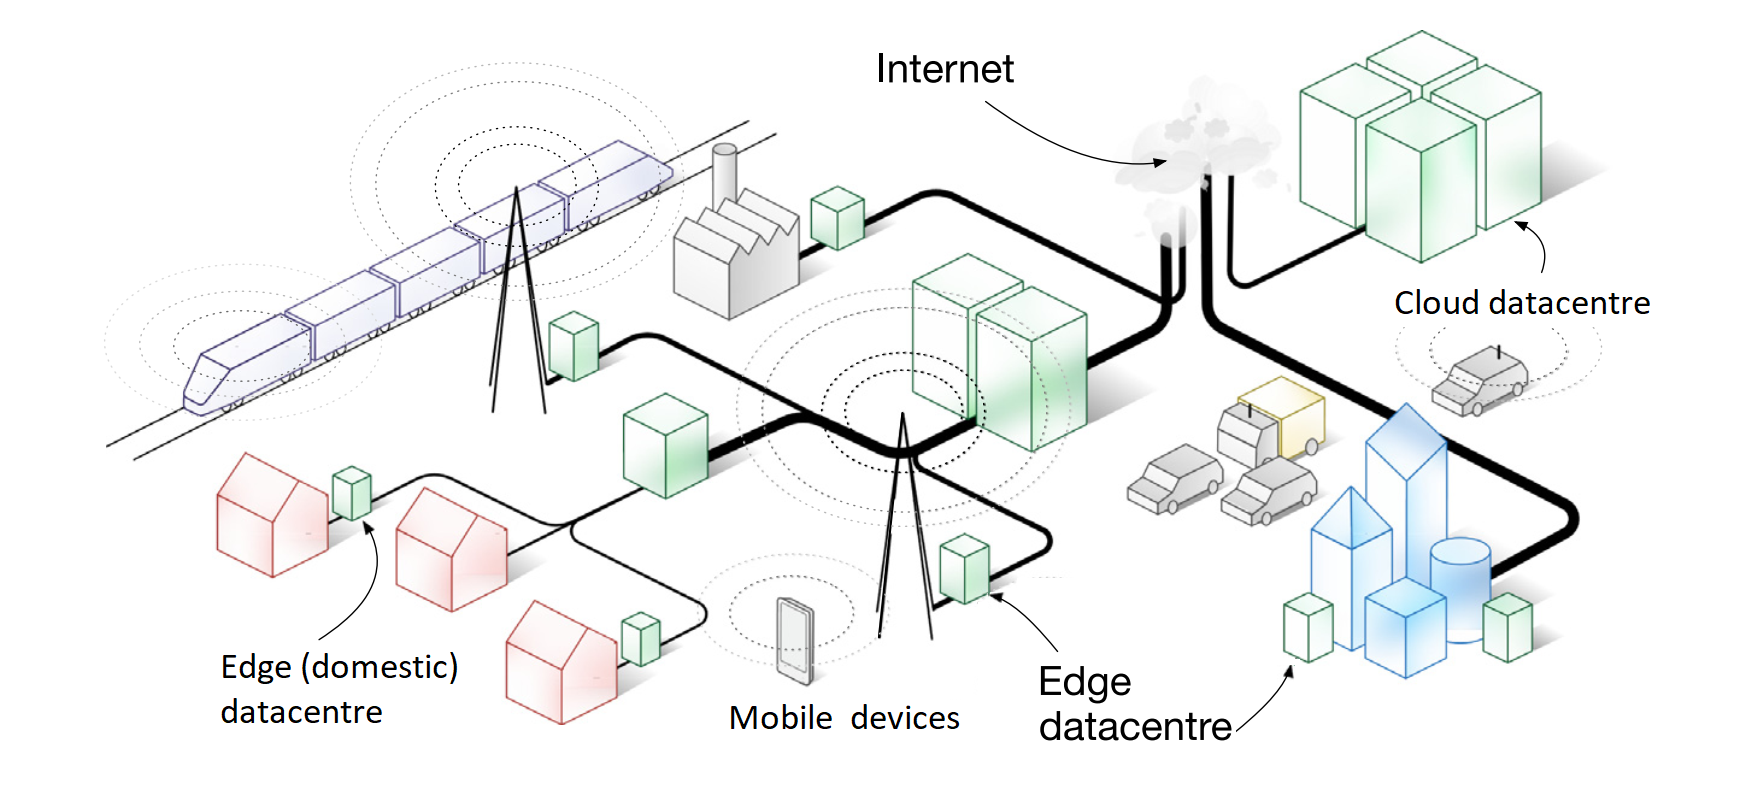
\includegraphics[width=0.9\textwidth]{figs/Continuum-overall.png}
	\caption{The computational continuum formed by coarsely distributed cloud datacenters, finely distributed edge datacenters, and mobile/IoT devices (adapted from~\cite{Tarneberg2017}).}
	\label{fig:continuum-overral}
\end{figure}

%\begin{figure}[tbp]
%	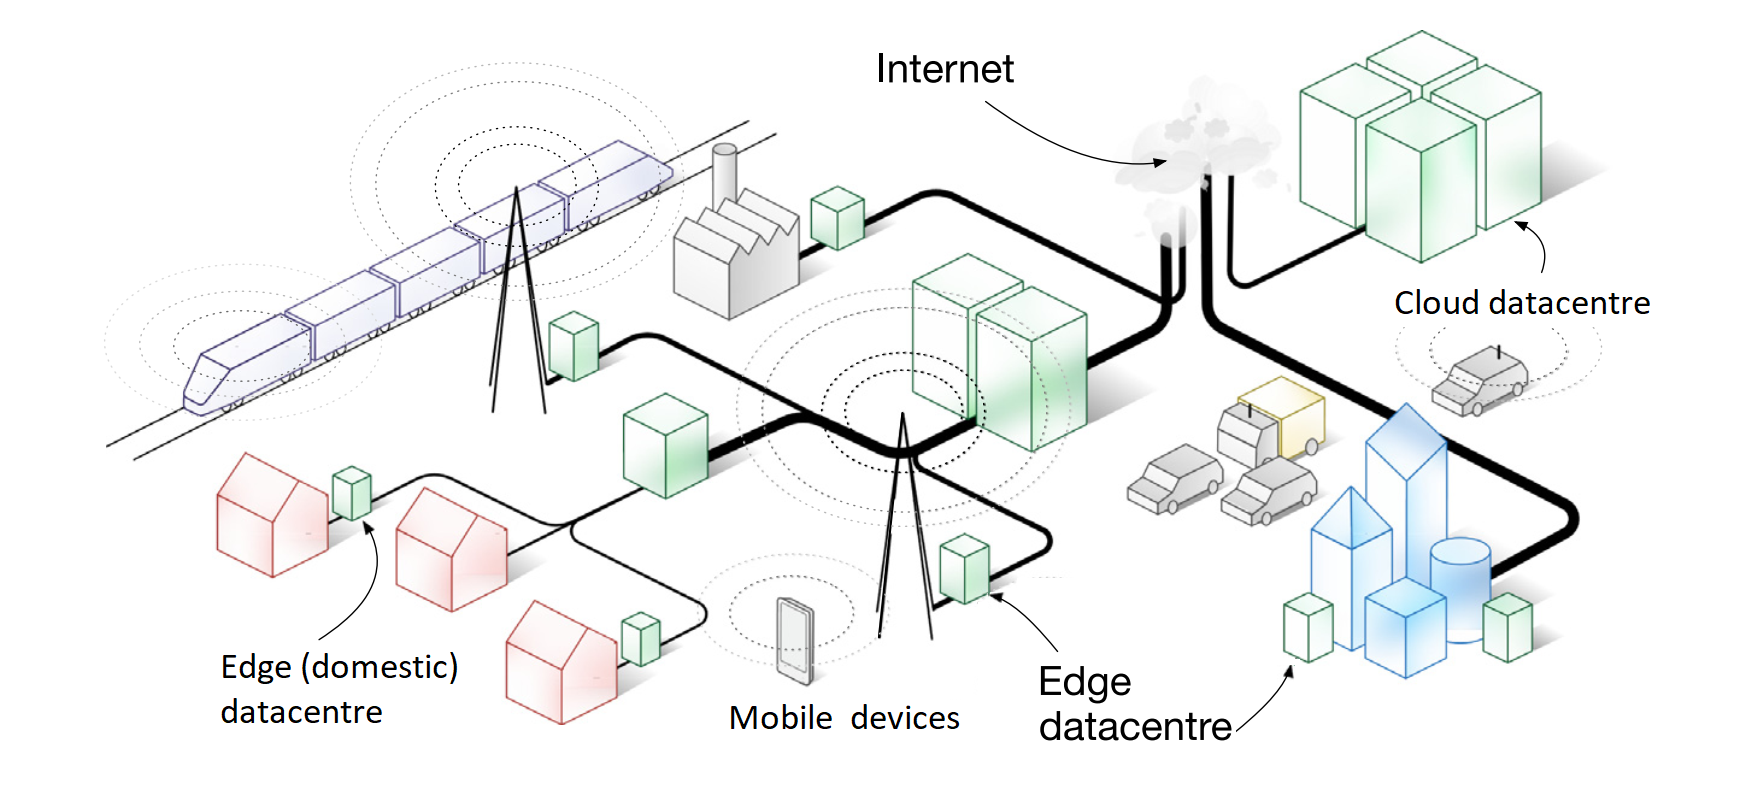
\includegraphics[width=0.9\textwidth]{figs/Continuum-overall.png}
%	\caption{The computational continuum formed by coarsely distributed cloud datacenters, finely distributed edge datacenters, and mobile/IoT devices.}
%	\label{fig:continuum-scenario}
%\end{figure}
 
%--- Last but not least, cloud servers should not be disregarded as a part of the Cloud-to-Edge continuum. %not sure whether to call it Cloud-to-Things or Cloud-to-Edge
%First, because client applications may still rely on Cloud backends for traditional, non delay-sensitive computation. Second, because edge servers may be unavailable from the certain locations. Thus, client applications must rely on a runtime mechanism to discover and negotiate the use of nearby edge infrastructure. As the alternative infrastructures (including the cloud) may exhibit uneven loads in different moments, the decision of which to use, must take into account their current status as well as the client application requirements in terms of latency and computational power. 


%Finally, to avoid increasing the burden of application development, computation to be executed at the edge should follow, to the extent possible, a common architecture and implementation with respect to its cloud counterpart. The same applies to the computation that may be offloaded from resource constrained devices to nearby edge infrastructure.  

%\subsection{Serverless Computing}

%Serverless computing~\cite{Roberts:2016, Hendrickson:2016}, also known as Functions-as-a-Service (FaaS)~\cite{MateosFaaster17}, emerged as an alternative execution model within cloud computing. In particular, its name derives from the fact that server management and capacity planning decisions are hidden from the software application engineers. Instead, third party providers of the serverless platform dynamically manage resource allocation and sharing for the execution of different types of computational tasks, known as \textit{functions}. Nowadays, all major cloud vendors provide serverless runtimes an associated ecosystem of services. 
%
%Among its main advantages, the serverless model is cost- and resource-efficient in comparison to virtual machine and container-based provisioning models, which generally involve significant periods of underutilization or idle time. In previous work~\cite{GarrigaMendonca2017}, we discussed the suitability of a serverless architecture to enable low-latency applications to use edge computing computational resources in an efficient, scalable and automated way. In this work, serverless computing is further explored in the realization of the computational continuum composed also by cloud and mobile devices by means of a unified model.

%mobile devices could make use of compute runtimes deployed at nearby edge servers to extend their capabilities. Notwithstanding the potential of such combination, a complete model for its realization is still missing~\cite{NasticServerlessEdge17}. 

\subsubsection*{Contributions of this Work}

%What: A3-E model as a contribution

In this paper, we propose a unified model for the realization of the computational continuum formed by cloud, edge, and mobile computing. At its core (and providing the name of the model) lies A3-E --- \textit{(A)wareness, (A)cquisition, (A)llocation and (E)ngagement} --- a flexible process targeting the efficient provisioning of computational resources from heterogeneous sources in the continuum to client applications featuring mixed requirements such as mobility, low-latency, and complex computation. 
%In specific, 
%What: A3-E and Serverless Computing 
%Targeting efficiency and scalability, 
A3-E proposes an automated management of service life-cycle by employing and extending the paradigm of serverless computing~\cite{Hendrickson:2016,baldini2017serverless,GarrigaMendonca2017}. In specific, A3-E explores the function-as-a-service (FaaS) execution model~\cite{MateosFaaster17} to allow stateless functions to be autonomously and opportunistically fetched, deployed and exposed as services with the twofold objective of achieving an efficient usage of computational resources needed for the realization of edge computing and consequently of the continuum. Additionally, A3-E encompasses the mutual client-server awareness and the dynamic placement of stateless computation along the continuum.

%The resulting suites both the resource limitations of edge computing and the autonomy degree required to release developers and infrastructure administrators from the burden of managing services life-cycle.


%and enables the realization of the continuum.

%What: The obtained results for latency and battery; other metrics?

As demonstrated through different experiments, an augmented reality application hosted by an Android platform device was able to rely on a client-side middleware implementing the A3-E process to proxy its requests to services dynamically selected from the continuum. In specific, these services were implemented as stateless functions that were executed in a cloud-based, edge-based, and mobile-based runtimes. The experiments have shown up to 90\% reduction of latency when edge services were used instead of cloud services, and a 74\% decrease of battery consumption when computation was offloaded from the Android device to edge servers. These results corroborate the importance of edge computing, as well as the feasibility of A3-E in the realization of the cloud-edge-mobile continuum.

%Finally, experiments with an augmented reality application have also shown the feasibility of A3-E model in the realization of the continuum, with a single client application been able to seamlessly alternate among local, edge, and cloud-based services.

% Such a selection is performed according to the application requirements (e.g., latency) and the actual context of the continuum as perceived by the client. 

%Last but not least, our contribution also includes a reference architecture for the realization of the proposed model. 

\subsubsection*{Paper Organization}

The rest of this paper is organized as follows. 
%Section~\ref{sec:motivation} describes the main motivation behind this work, including application scenarios and the computational continuum.  
Section~\ref{sec:background} provides a brief background on the main topics and concepts used by this work. Section~\ref{sec:continuum} details our concept of a cloud-edge-mobile continuum and specifies requirements for its realization. Section~\ref{sec:proposal} provides a detailed description of the A3-E model, whereas Section~\ref{sec:implementation} details both the client-side implementation for Android platform and the server-side implementation for edge-computing. Section~\ref{sec:evaluation} reports on the experiments performed to evaluate our proposal with an augment reality application. Section~\ref{sec:related} presents related work. Finally, Section~\ref{sec:conclusions} concludes the paper and delineates future work.




